\documentclass[tikz]{standalone}
\usepackage{tikz}
\usepackage{bm}

\definecolor{myblue}{RGB}{210,237,252} % Custom blue color
\definecolor{myblue2}{RGB}{18,131,200} % Custom blue color
\definecolor{myred}{RGB}{248,178,190} % Custom red color
\definecolor{myyellow}{RGB}{252,246,200} % Custom yellow color


\begin{document}
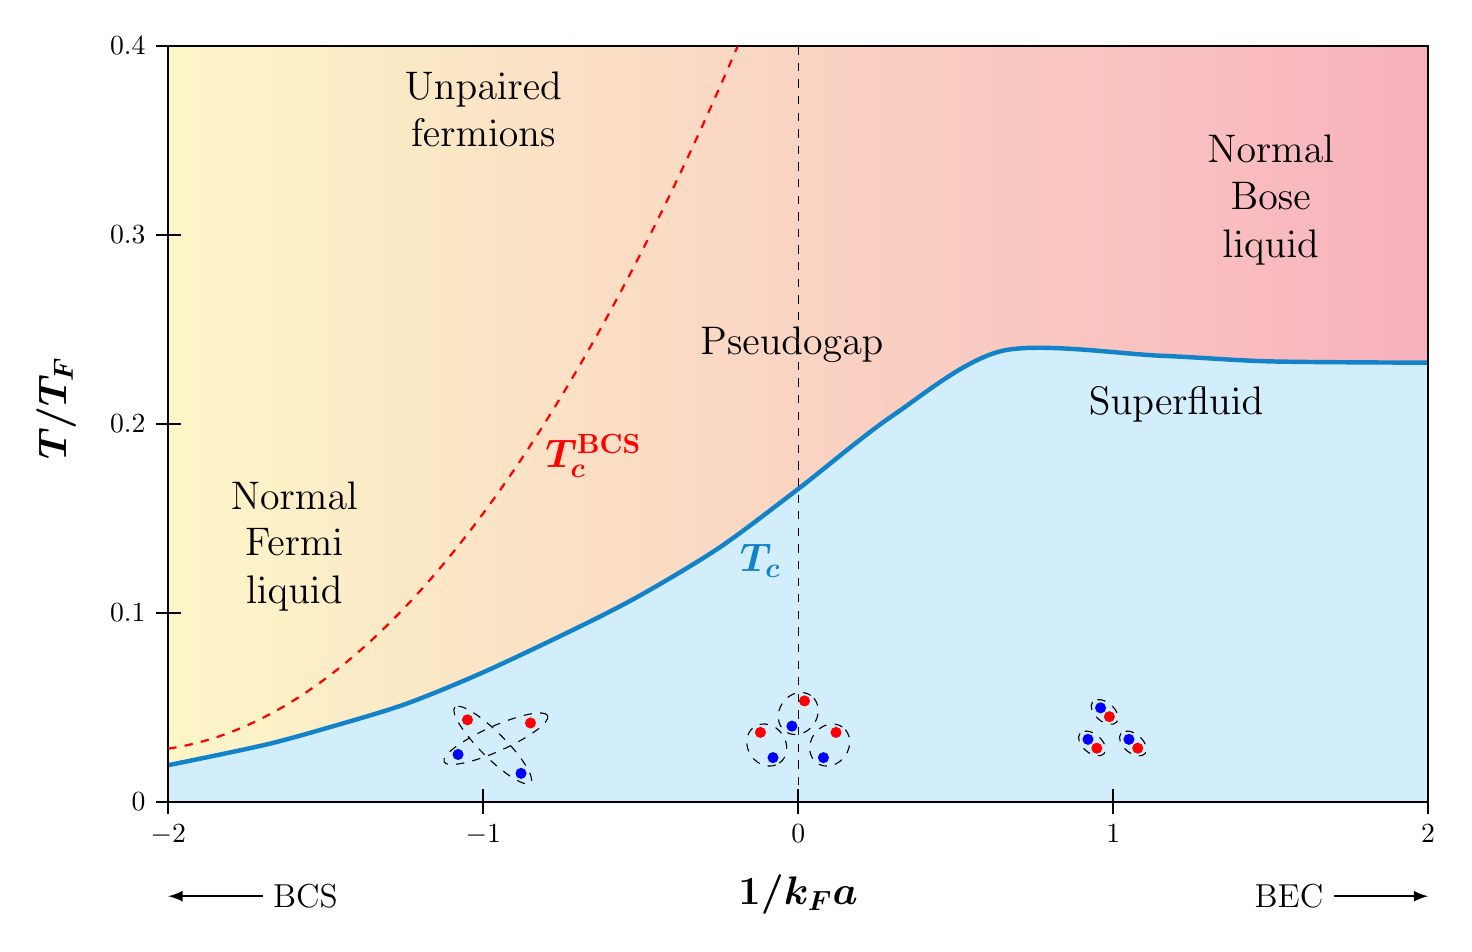
\begin{tikzpicture}[scale=4]
  % Color gradient
  \shade[left color=myyellow, right color=myred] (-2,0) rectangle (2,2.4);

  % Shading below the blue line
  \fill[myblue] (-2,0.116) plot [smooth] coordinates {(-2,0.116) (-1.7,0.179) (-1.5,0.233) (-1.25,0.309) (-1,0.411) (-0.71,0.548) (-0.5,0.656) (-0.25,0.807) (0,0.993) (0.3,1.226) (0.65,1.432) (1.15,1.416) (1.5,1.398) (2,1.394)} -- (2,0) -- (-2,0) -- cycle;

  % Curved blue line
  \draw[myblue2,ultra thick] plot [smooth] coordinates {(-2,0.116) (-1.7,0.179) (-1.5,0.233) (-1.25,0.309) (-1,0.411) (-0.71,0.548) (-0.5,0.656) (-0.25,0.807) (0,0.993) (0.3,1.226) (0.65,1.432) (1.15,1.416) (1.5,1.398) (2,1.394)};
  
  % Box
  \draw[thick] (-2,0) rectangle (2,2.4);

  % X-axis ticks and labels
  \foreach \x in {-2,-1,0,1,2}
    \draw[thick] (\x,0.04) -- (\x,-0.04) node[below] {$\x$};

  % Y-axis ticks and labels
  \draw[thick] (-1.96,0.0) -- (-2.04,0.0) node[left] {$0$};
  \draw[thick] (-1.96,0.6) -- (-2.04,0.6) node[left] {$0.1$};
  \draw[thick] (-1.96,1.2) -- (-2.04,1.2) node[left] {$0.2$};
  \draw[thick] (-1.96,1.8) -- (-2.04,1.8) node[left] {$0.3$};
  \draw[thick] (-1.96,2.4) -- (-2.04,2.4) node[left] {$0.4$};
  
  % Annotation
  \node[below,thick] at (0,-0.2) {\Large{$\bm{1/k_Fa}$}};
  \node[below,thick,rotate=90] at (-2.45,1.25) {\Large{$\bm{T/T_F}$}};
  \draw[latex-,thick] (-2,-0.3) -- (-1.7,-0.3) node[right] {\large{BCS}};
  \draw[latex-,thick] (2,-0.3) -- (1.7,-0.3) node[left] {\large{BEC}};
  \node[myblue2,below,thick] at (-0.12,0.85) {\Large{$\bm{T_c}$}};
  \node[red,below,thick] at (-0.65,1.2) {\Large{$\bm{T^{\mathrm{BCS}}_c}$}};
  \node[below,thick] at (1.2,1.35) {\Large{Superfluid}};
  \node[below,thick] at (-1.6,1.05) {\Large{Normal}};
  \node[below,thick] at (-1.6,0.90) {\Large{Fermi}};
  \node[below,thick] at (-1.6,0.75) {\Large{liquid}};
  \node[below,thick] at (-0.02,1.54) {\Large{Pseudogap}};
  \node[below,thick] at (-1.0,2.35) {\Large{Unpaired}};
  \node[below,thick] at (-1.0,2.20) {\Large{fermions}};
  \node[below,thick] at (1.5,2.15) {\Large{Normal}};
  \node[below,thick] at (1.5,2.00) {\Large{Bose}};
  \node[below,thick] at (1.5,1.85) {\Large{liquid}};
  
  % Vertical dashed line
  \draw[dashed] (0,0) -- (0,2.4);
  
  % Red dashed line
 \draw[domain=-2:-0.192, samples=200, variable=\x, red, thick, dashed] plot(\x, {(\x+2.12)^2/1.66+0.16});
  
  % Small circles
  \fill[red] (-0.85,0.25) circle (0.5pt);
  \fill[blue] (-0.88,0.09) circle (0.5pt);
  \fill[red] (-1.05,0.26) circle (0.5pt);
  \fill[blue] (-1.08,0.15) circle (0.5pt);
  \fill[red] (0.12,0.22) circle (0.5pt);
  \fill[blue] (0.08,0.14) circle (0.5pt);
  \fill[red] (-0.12,0.22) circle (0.5pt);
  \fill[blue] (-0.08,0.14) circle (0.5pt);
  \fill[red] (0.02,0.32) circle (0.5pt);
  \fill[blue] (-0.02,0.24) circle (0.5pt);
  \fill[red] (0.948,0.17) circle (0.5pt);
  \fill[blue] (0.92,0.198) circle (0.5pt);
  \fill[red] (1.078,0.17) circle (0.5pt);
  \fill[blue] (1.05,0.198) circle (0.5pt);
  \fill[red] (0.988,0.27) circle (0.5pt);
  \fill[blue] (0.96,0.298) circle (0.5pt);
  
  % Dashed ellipse
  \draw[dashed, rotate around={24:(-0.96,0.2)}, shift={(-0.96,0.2)}] (0,0) ellipse (0.18 and 0.04);
  \draw[dashed, rotate around={135:(-0.97,0.18)}, shift={(-0.97,0.18)}] (0,0) ellipse (0.17 and 0.04);
  \draw[dashed, rotate around={55:(0.1,0.18)}, shift={(0.1,0.18)}] (0,0) ellipse (0.07 and 0.06);
  \draw[dashed, rotate around={-55:(-0.1,0.18)}, shift={(-0.1,0.18)}] (0,0) ellipse (0.07 and 0.06);
  \draw[dashed, rotate around={55:(0,0.28)}, shift={(0,0.28)}] (0,0) ellipse (0.07 and 0.06);
  \draw[dashed, rotate around={140:(0.933,0.185)}, shift={(0.933,0.185)}] (0,0) ellipse (0.05 and 0.03);
  \draw[dashed, rotate around={140:(0.973,0.285)}, shift={(0.973,0.285)}] (0,0) ellipse (0.05 and 0.03);
  \draw[dashed, rotate around={140:(1.063,0.185)}, shift={(1.063,0.185)}] (0,0) ellipse (0.05 and 0.03);
  
\end{tikzpicture}
\end{document}